\documentclass[journal]{IEEEtran}
\usepackage{cite}
\usepackage{amsmath,amssymb,amsfonts}
\usepackage{algorithmic}
\usepackage{algorithm}
\usepackage{graphicx}
\usepackage{textcomp}
\usepackage{xcolor}
\usepackage{booktabs}
\usepackage{multirow}
\usepackage{hyperref}
\usepackage{bm}
\usepackage{epstopdf}


\begin{document}

\title{APEX: Adaptive Phase-Aware Exploration for Lightweight Client Selection in Federated Learning}

\author{
% Authors to be added
}

\maketitle

\begin{abstract}
Selecting the right clients in each communication round is an important problem in Federated Learning (FL), especially when client data is non-identically distributed (non-IID). Most existing client selection methods focus on either selecting high-loss clients to speed up convergence, or selecting diverse clients to reduce gradient noise. However, none of them address both aspects together in a lightweight manner. In this paper, a phase-aware client selection algorithm called Adaptive Phase-Aware Exploration (APEX) is proposed for FL under non-IID data. The proposed method combines contextual Thompson sampling with a label-histogram-based diversity proxy to score and select clients. A phase detector based on loss trajectory analysis automatically switches between diversity-focused and exploitation-focused selection, with hysteresis to prevent rapid phase oscillation. In addition, a heterogeneity-aware scaling mechanism based on Jensen-Shannon divergence adjusts the diversity weight according to the data distribution across clients, removing the need for manual tuning. The proposed algorithm has zero trainable parameters and adds only 3.9~ms of per-round computational overhead. Experimental results on CIFAR-10, CIFAR-100, MNIST, and Fashion-MNIST with ResNet18 over 200 communication rounds demonstrate that APEX achieves 70.67\% test accuracy on CIFAR-10 under Dirichlet non-IID partitioning ($\alpha = 0.3$), ranking first among eight baseline methods across three independent seeds, with $4\times$ better participation fairness than system-aware baselines. It is observed that the performance advantage of the proposed method increases with heterogeneity severity, achieving 14.4 percentage points above Oort at $\alpha = 0.1$.
\end{abstract}

{\noindent\small\bfseries\textit{Impact Statement}---Federated learning allows multiple devices to collaboratively train a machine learning model without sharing their private data. A key practical challenge is deciding which devices should participate in each round of training. Poor selection leads to slow convergence, biased models, and unfair resource usage among participants. The algorithm proposed in this paper selects devices by combining lightweight statistical exploration with an automatic phase detection mechanism that adapts the selection strategy as training progresses. On standard benchmarks across four datasets and three heterogeneity levels, the proposed method ranks first among eight baselines in 8 out of 9 settings and achieves $4\times$ fairer participation compared to system-aware methods, with negligible computational overhead. These results are directly applicable to federated deployments in healthcare monitoring, mobile networks, and Internet of Things systems, where communication budgets are limited and equitable device participation is a practical necessity.\par}

\begin{IEEEkeywords}
Federated learning, client selection, Thompson sampling, non-IID data, phase-aware learning, gradient diversity.
\end{IEEEkeywords}

\section{Introduction}

\IEEEPARstart{B}{EING} recognized as a promising distributed learning algorithm, Federated Learning (FL) \cite{mcmahan2017communication} is able to decouple the processes of data acquisition and computation. In FL, multiple clients train a shared model collaboratively without sharing their raw data with a central server. Such privacy-preserving nature has been investigated in existing literature \cite{kairouz2021advances}, \cite{li2020federated}, \cite{mai2024study}. In each communication round, the server selects a subset of clients, the selected clients train on their local data, and the updated parameters are sent back to the server for aggregation.

One important research direction in FL is the problem of client selection \cite{cho2022towards}, \cite{lai2021oort}, \cite{balakrishnan2022diverse}, \cite{huang2024active}. When client data distributions are non-identical (non-IID), selecting the right clients in each round has a large effect on convergence speed and final model quality. The convergence bound for FedAvg \cite{li2020federated} contains a client drift term caused by non-IID data and a gradient variance term caused by partial participation. Reducing both terms at the same time is needed for fast convergence.

Several methods have been proposed for client selection in FL. In \cite{cho2022towards}, Power-of-Choice selects clients with high training loss, achieving up to $3\times$ faster convergence. In \cite{balakrishnan2022diverse}, DivFL selects diverse clients using submodular maximization over gradients. However, Power-of-Choice does not consider diversity, and DivFL requires all client gradients to be communicated. In \cite{tang2022fedcor}, FedCor models loss correlations using a Gaussian process with $\mathcal{O}(N^2)$ cost. System-aware methods such as FedCS \cite{nishio2019client}, TiFL \cite{chai2020tifl}, and Oort \cite{lai2021oort} improve wall-clock time but tend to select the same clients repeatedly. Reinforcement learning based methods \cite{wang2020optimizing}, \cite{zheng2024fedaeb}, \cite{dai2025fedhrl}, \cite{ning2024fedgcs} show good results but require training neural networks with considerable overhead. Thompson sampling \cite{thompson1933likelihood}, \cite{chapelle2011empirical} has been applied as a lighter alternative with regret guarantees \cite{agrawal2012analysis}, but existing approaches use only a single reward signal. In \cite{yan2023criticalfl}, it is shown that FL training exhibits critical learning periods where gradient errors cause large accuracy drops, but the proposed CriticalFL framework is not a standalone selector.

\subsection{Contributions}
In this paper, we propose APEX (Adaptive Phase-aware EXploration), a lightweight client selection algorithm for FL with non-IID data. Unlike the existing works listed in \cite{cho2022towards}, \cite{lai2021oort}, \cite{balakrishnan2022diverse}, \cite{wang2020optimizing}, \cite{zheng2024fedaeb}, \cite{dai2025fedhrl}, \cite{ning2024fedgcs}, where the selection strategy is either loss-biased or diversity-aware but not both, we combine contextual Thompson sampling with a label-histogram-based diversity proxy while keeping zero trainable parameters. To the best of authors' knowledge, we are the first to address loss-biased selection, gradient diversity, phase adaptation, and heterogeneity calibration together in a single lightweight framework. The main contributions of this paper can be summarized as follows.

\begin{enumerate}
    \item \textit{Phase-Aware Client Selection Framework:} We design a client selection algorithm that combines contextual Thompson sampling with a label-histogram-based diversity proxy. A phase detector based on loss trajectory analysis is introduced to automatically switch between diversity-focused and exploitation-focused selection, with hysteresis and minimum dwell time to prevent rapid switching.

    \item \textit{Heterogeneity-Aware Scaling:} We propose a scaling mechanism that computes the Jensen-Shannon divergence \cite{lin1991divergence} across client label distributions and adjusts the diversity weight accordingly. This removes the need for manual tuning across different heterogeneity levels.

    \item \textit{Posterior Regularization:} A decaying variance floor is introduced to prevent early posterior collapse. In addition, a confidence-aware blending parameter is used so that new clients are scored by contextual features, while well-observed clients get a stronger Thompson sampling influence.

    \item \textit{Experimental Analysis:} Extensive simulations are carried out on CIFAR-10, CIFAR-100, MNIST, and Fashion-MNIST across eight baselines, three heterogeneity levels ($\alpha \in \{0.1, 0.3, 0.6\}$), three federation scales ($N \in \{50, 100, 200\}$), and three independent seeds per setting. It is observed that APEX achieves 70.67\% on CIFAR-10 under non-IID partitioning ($\alpha = 0.3$), ranking first among eight methods, with $4\times$ better participation fairness than system-aware baselines. A component analysis is also conducted to assess the stability contribution of each mechanism.
\end{enumerate}

\textit{Organization:} The rest of this paper is organized as follows. Section~II reviews related work on client selection in FL. Section~III details the system model and problem formulation. The proposed APEX algorithm is described in Section~IV, followed by theoretical analysis in Section~V. Experimental results are presented in Section~VI. Section~VII concludes this paper and Section~VIII discusses future research directions.

% ============================================================================
% SECTION II: RELATED WORK
% ============================================================================
\section{Related Work}

Client selection in FL has been studied from several directions. In this section, the main approaches are reviewed and their limitations are discussed.

\subsection{Loss-Based and Utility-Based Selection}

In \cite{cho2022towards}, a biased client selection strategy called Power-of-Choice is proposed, where a random subset of clients report their local training losses and the server selects the ones with the highest loss. It is shown that this approach reduces convergence time by up to $3\times$. The method does not, however, account for gradient diversity among the selected clients. Similarly, the work in \cite{lai2021oort} proposes Oort, which combines a statistical utility score based on training loss with a system utility score based on the client's computation and communication speed. An exploration bonus is used to avoid selecting the same clients repeatedly. On the other hand, the system utility component favours faster clients, which reduces participation fairness over time.

\subsection{Diversity-Based Selection}

In \cite{balakrishnan2022diverse}, a diversity-based method called DivFL is proposed, where client selection is formulated as a submodular facility location problem over gradients. Strong approximation guarantees are provided. DivFL requires, however, all $N$ client gradients to be communicated every round, leading to $\mathcal{O}(N \cdot d)$ overhead. Likewise, in \cite{hu2025fedgscs}, a gradient similarity-based method is proposed where clients most aligned with the global gradient direction are selected. Results show up to 80\% fewer communication rounds, but the method also requires $\mathcal{O}(N \cdot d)$ gradient communication. In \cite{carbonara2024mmr}, a Maximal Marginal Relevance-based approach (MMR-Diverse) is proposed, where a loss-sorted candidate pool is re-ranked using the cosine similarity of client gradient proxies. While MMR-Diverse achieves competitive results under moderate heterogeneity, it does not adapt its strategy to the training phase and degrades under extreme non-IID conditions, as observed in our experiments.

\subsection{Bandit and Learning-Based Methods}

Thompson sampling \cite{thompson1933likelihood} is a Bayesian approach to the multi-armed bandit problem with $\mathcal{O}(\sqrt{NT\log T})$ regret bounds \cite{agrawal2012analysis}. When applied to FL, it maintains a posterior estimate of each client's contribution and selects clients by sampling from these posteriors. Existing approaches, however, use only a single reward signal without multi-dimensional context. The work in \cite{ma2025fnns} proposes FNNS, a combinatorial neural contextual bandit with $\mathcal{O}(N \cdot h)$ overhead. On the reinforcement learning side, FAVOUR \cite{wang2020optimizing} uses a DDQN agent, FedAEB \cite{zheng2024fedaeb} uses Soft Actor-Critic, FedGCS \cite{ning2024fedgcs} uses a generative encoder-decoder, and in \cite{dai2025fedhrl} a transformer pointer network is proposed. While these methods show improvements, they require training neural networks with $\mathcal{O}(N^2)$ or $\mathcal{O}(N \cdot d)$ complexity.

\subsection{Phase-Aware and System-Aware Methods}

The concept of critical learning periods (CLPs) is introduced for FL in \cite{yan2023criticalfl}. Gradient errors during CLPs cause accuracy drops of up to $100\times$ the magnitude observed in non-critical periods. CriticalFL detects CLPs and augments any existing selector, but it is not a standalone method. In \cite{nishio2019client}, FedCS selects the maximum number of clients that can complete training within a given deadline. Similarly, in \cite{chai2020tifl}, TiFL groups clients into tiers based on training speed. Both improve wall-clock time but tend to repeatedly select the same fast clients, resulting in Gini coefficients exceeding 0.79 in our experiments. The work in \cite{tang2022fedcor} proposes FedCor, which models loss correlations using a Gaussian process with $\mathcal{O}(N^2)$ cost per round.

\subsection{Summary of Gaps}

In Table~\ref{tab:gap_analysis}, we summarize and compare the features of existing client selection methods. The impact of data heterogeneity on FL performance has been systematically studied in \cite{vahidian2024rethinking}, where new notions and standard benchmarks for non-IID evaluation are introduced. It can be witnessed that no existing method combines loss-biased selection with gradient diversity, adapts its strategy based on the training phase, and self-calibrates to the heterogeneity level, all with zero trainable parameters. We propose APEX to address these gaps with $\mathcal{O}(NK^2L)$ per-round complexity.

\begin{table}[t]
\centering
\caption{Comparison of client selection methods ($L$ = number of label classes).}
\label{tab:gap_analysis}
\footnotesize
\renewcommand{\arraystretch}{1.05}
\setlength{\tabcolsep}{2.5pt}
\begin{tabular}{lcccccc}
\toprule
\textbf{Method} & \textbf{Loss} & \textbf{Div.} & \textbf{Phase} & \textbf{Calib.} & \textbf{Params.} & \textbf{Cost} \\
\midrule
PoC \cite{cho2022towards} & \checkmark & -- & -- & -- & 0 & $O(d)$ \\
Oort \cite{lai2021oort} & \checkmark & -- & -- & -- & 0 & $O(N)$ \\
DivFL \cite{balakrishnan2022diverse} & -- & \checkmark & -- & -- & 0 & $O(Nd)$ \\
FedGSCS \cite{hu2025fedgscs} & -- & \checkmark & -- & -- & 0 & $O(Nd)$ \\
MMR-Div. \cite{carbonara2024mmr} & \checkmark & \checkmark & -- & -- & 0 & $O(Nd)$ \\
FedCor \cite{tang2022fedcor} & \checkmark & -- & -- & -- & $O(N^2)$ & $O(N^2)$ \\
FAVOUR \cite{wang2020optimizing} & \checkmark & -- & -- & -- & $O(Nd)$ & $O(Nd)$ \\
FedAEB \cite{zheng2024fedaeb} & \checkmark & -- & -- & -- & $O(Nd)$ & $O(Nd)$ \\
FedHRL \cite{dai2025fedhrl} & \checkmark & -- & -- & -- & $O(N^2)$ & $O(N^2)$ \\
FedGCS \cite{ning2024fedgcs} & \checkmark & -- & -- & -- & $O(Nd)$ & $O(Nd)$ \\
FNNS \cite{ma2025fnns} & \checkmark & -- & -- & -- & $O(Nh)$ & $O(Nh)$ \\
CriticalFL \cite{yan2023criticalfl} & -- & -- & \checkmark & -- & 0 & $O(1)$ \\
FedCS \cite{nishio2019client} & -- & -- & -- & -- & 0 & $O(N)$ \\
TiFL \cite{chai2020tifl} & -- & -- & -- & -- & 0 & $O(N)$ \\
\midrule
\textbf{APEX} & \checkmark & \checkmark & \checkmark & \checkmark & \textbf{0} & $O(NK^2L)$ \\
\bottomrule
\end{tabular}
\end{table}

% ============================================================================
% SECTION III: SYSTEM MODEL AND PROBLEM FORMULATION
% ============================================================================
\section{System Model and Problem Formulation}

In this section, the federated learning setup is described first. The convergence bound under non-IID data is then presented to motivate the client selection problem. Finally, the problem statement is formulated.

\subsection{Federated Learning Setup}

We consider a federated learning system with $N$ clients and a central server. The $n^{th}$ client stores a local private dataset $\mathcal{D}_n = \{(\bm{x}_i, y_i)\}_{i=1}^{|\mathcal{D}_n|}$, where $\bm{x}_i$ is the input data and $y_i$ is the corresponding label. The datasets are not shared with the server. The total dataset across all clients is $\mathcal{D} = \bigcup_{n=1}^{N} \mathcal{D}_n$ with size $D = \sum_{n=1}^{N} |\mathcal{D}_n|$.

The local loss function for client $n$ can be written as
\begin{equation}
L_n(\bm{w}) = \frac{1}{|\mathcal{D}_n|} \sum_{(\bm{x}_i, y_i) \in \mathcal{D}_n} \ell(\bm{w}; \bm{x}_i, y_i),
\label{eq:local_loss}
\end{equation}
where $\bm{w}$ denotes the model parameters and $\ell(\cdot)$ is the per-sample loss. The objective of the server is to minimize the weighted sum of local losses, that is,
\begin{equation}
\min_{\bm{w}} \; F(\bm{w}) = \sum_{n=1}^{N} \frac{|\mathcal{D}_n|}{D} L_n(\bm{w}).
\label{eq:global_obj}
\end{equation}

Training proceeds over $T$ communication rounds. In each round $t$, the server selects a subset $\mathcal{S}_t \subset \{1, 2, \ldots, N\}$ with $|\mathcal{S}_t| = K$. Each selected client $n \in \mathcal{S}_t$ initializes from the current global model and performs $E$ local epochs of stochastic gradient descent (SGD), each epoch comprising $\tau_n = \lceil |\mathcal{D}_n|/B \rceil$ mini-batch steps (with batch size $B$). Denoting the total number of local steps as $Q_n = E\tau_n$, the local update recursion is
\begin{equation}
\begin{split}
\bm{w}_{n,t}^{(0)} &= \bm{w}_t, \\
\bm{w}_{n,t}^{(k+1)} &= \bm{w}_{n,t}^{(k)} - \eta \nabla \tilde{L}_n\!\bigl(\bm{w}_{n,t}^{(k)}\bigr),\; k = 0, \ldots, Q_n\!-\!1,
\end{split}
\label{eq:local_update}
\end{equation}
where $\eta$ is the local learning rate and $\nabla \tilde{L}_n$ denotes the stochastic mini-batch gradient of client $n$. The model returned to the server is $\bm{w}_{n,t+1} = \bm{w}_{n,t}^{(Q_n)}$. Note that for $k \geq 1$ the gradients are evaluated at $\bm{w}_{n,t}^{(k)} \neq \bm{w}_t$; this is the source of the client drift discussed below. The server then aggregates the local models using the FedAvg rule \cite{mcmahan2017communication}, and the updated global model can be written as
\begin{equation}
\bm{w}_{t+1} = \sum_{n \in \mathcal{S}_t} \frac{|\mathcal{D}_n|}{\sum_{j \in \mathcal{S}_t} |\mathcal{D}_j|} \bm{w}_{n,t+1}.
\label{eq:fedavg}
\end{equation}

To simulate non-IID data distributions across clients, the Dirichlet partition method \cite{hsu2019measuring}, \cite{vahidian2024rethinking} is used. Each client receives samples drawn according to a Dirichlet distribution $\text{Dir}(\alpha)$ over the label space. A smaller value of $\alpha$ produces more heterogeneous partitions.

\subsection{Convergence Bound and Client Selection}

Under non-IID data, the convergence of FedAvg is bounded as shown in \cite{li2020federated}, \cite{karimireddy2020scaffold}. For $\mu$-strongly convex and $\psi$-smooth local objectives, the convergence bound after $T$ rounds can be given as
\begin{equation}
\mathbb{E}\left[\|\bm{w}_T - \bm{w}^*\|_2^2\right] \leq (1 - \eta\mu)^T \|\bm{w}_0 - \bm{w}^*\|_2^2 + A \Gamma + \frac{B \sigma^2}{K},
\label{eq:convergence_bound}
\end{equation}
where $\bm{w}^*$ is the global optimum, $A$ and $B$ are positive constants that depend on the learning rate $\eta$, smoothness $\psi$, and strong convexity $\mu$. The terms $\Gamma$ and $\sigma^2$ are defined below.

The term $\Gamma$ is the client drift, which measures the deviation of local objectives from the global objective. Following the bounded gradient dissimilarity framework in \cite{karimireddy2020scaffold}, it is given by
\begin{equation}
\Gamma = \sum_{n=1}^{N} \frac{|\mathcal{D}_n|}{D} \|\nabla L_n(\bm{w}^*)\|_2^2.
\label{eq:client_drift}
\end{equation}
Under IID data, $\Gamma = 0$ since all local objectives share the same minimizer. Under non-IID data, $\Gamma > 0$ and it increases with the heterogeneity level.

The term $\sigma^2/K$ captures gradient variance due to partial participation. When only $K$ out of $N$ clients participate in each round, the aggregated gradient is a noisy estimate of the full gradient. The variance $\sigma^2$ can be written as
\begin{equation}
\sigma^2 = \frac{1}{N} \sum_{n=1}^{N} \mathbb{E}\left[\|\nabla L_n(\bm{w}) - \nabla F(\bm{w})\|_2^2\right].
\label{eq:grad_variance}
\end{equation}

From (\ref{eq:convergence_bound}), fast convergence requires reducing the effective impact of both $\Gamma$ and $\sigma^2/K$. Selecting clients with high training loss reduces the effective contribution of $\Gamma$ by prioritizing clients far from their local optimum \cite{cho2022towards}. On the other hand, selecting clients with diverse gradients reduces the effective gradient variance \cite{balakrishnan2022diverse}. This convergence behavior under non-IID conditions has been further studied in \cite{mai2024study}, where server-side learning is shown to mitigate performance degradation caused by data heterogeneity. However, no existing lightweight method addresses both terms at the same time.

\subsection{Problem Statement}

The goal is to find a client selection policy $\pi$ that selects $K$ clients in each round $t$ to minimize the right-hand side of (\ref{eq:convergence_bound}). The problem can be formulated as
\begin{equation}
\min_{\pi} \; \mathbb{E}\left[\|\bm{w}_T - \bm{w}^*\|_2^2\right]
\label{eq:problem}
\end{equation}
subject to the following constraints:
\begin{enumerate}
    \item $|\mathcal{S}_t| = K$ for all $t = 1, \ldots, T$,
    \item No client gradient communication is required for selection,
    \item The per-client selection overhead is $\mathcal{O}(1)$ with respect to the model dimension $d$.
\end{enumerate}

Constraint 1 fixes the communication budget per round. Constraint 2 rules out methods such as DivFL \cite{balakrishnan2022diverse} that require $\mathcal{O}(N \cdot d)$ gradient uploads. Constraint 3 rules out methods such as FedCor \cite{tang2022fedcor} that require $\mathcal{O}(N^2)$ computation per round. The proposed APEX algorithm satisfies all three constraints while targeting both the $\Gamma$ and $\sigma^2/K$ terms in (\ref{eq:convergence_bound}).


% ============================================================================
% SECTION IV: PROPOSED APEX ALGORITHM
% ============================================================================
\section{Proposed APEX Algorithm}

In this section, we present the proposed APEX algorithm, where the main design idea is to combine loss-biased selection with gradient diversity in a phase-adaptive manner, while keeping zero trainable parameters. The overall framework of the proposed method is illustrated in Fig.~\ref{fig:system_model}. The phase detection mechanism with hysteresis is discussed first. Subsequently, the contextual Thompson sampling component with posterior regularization is presented. The heterogeneity-aware gradient diversity proxy is then described, followed by the phase-adaptive score combination. The complete algorithm is summarized in Algorithm~\ref{alg:apex}.

\begin{figure*}[t]
\centering
%\includegraphics[width=0.95\textwidth]{figures/system_model.pdf}
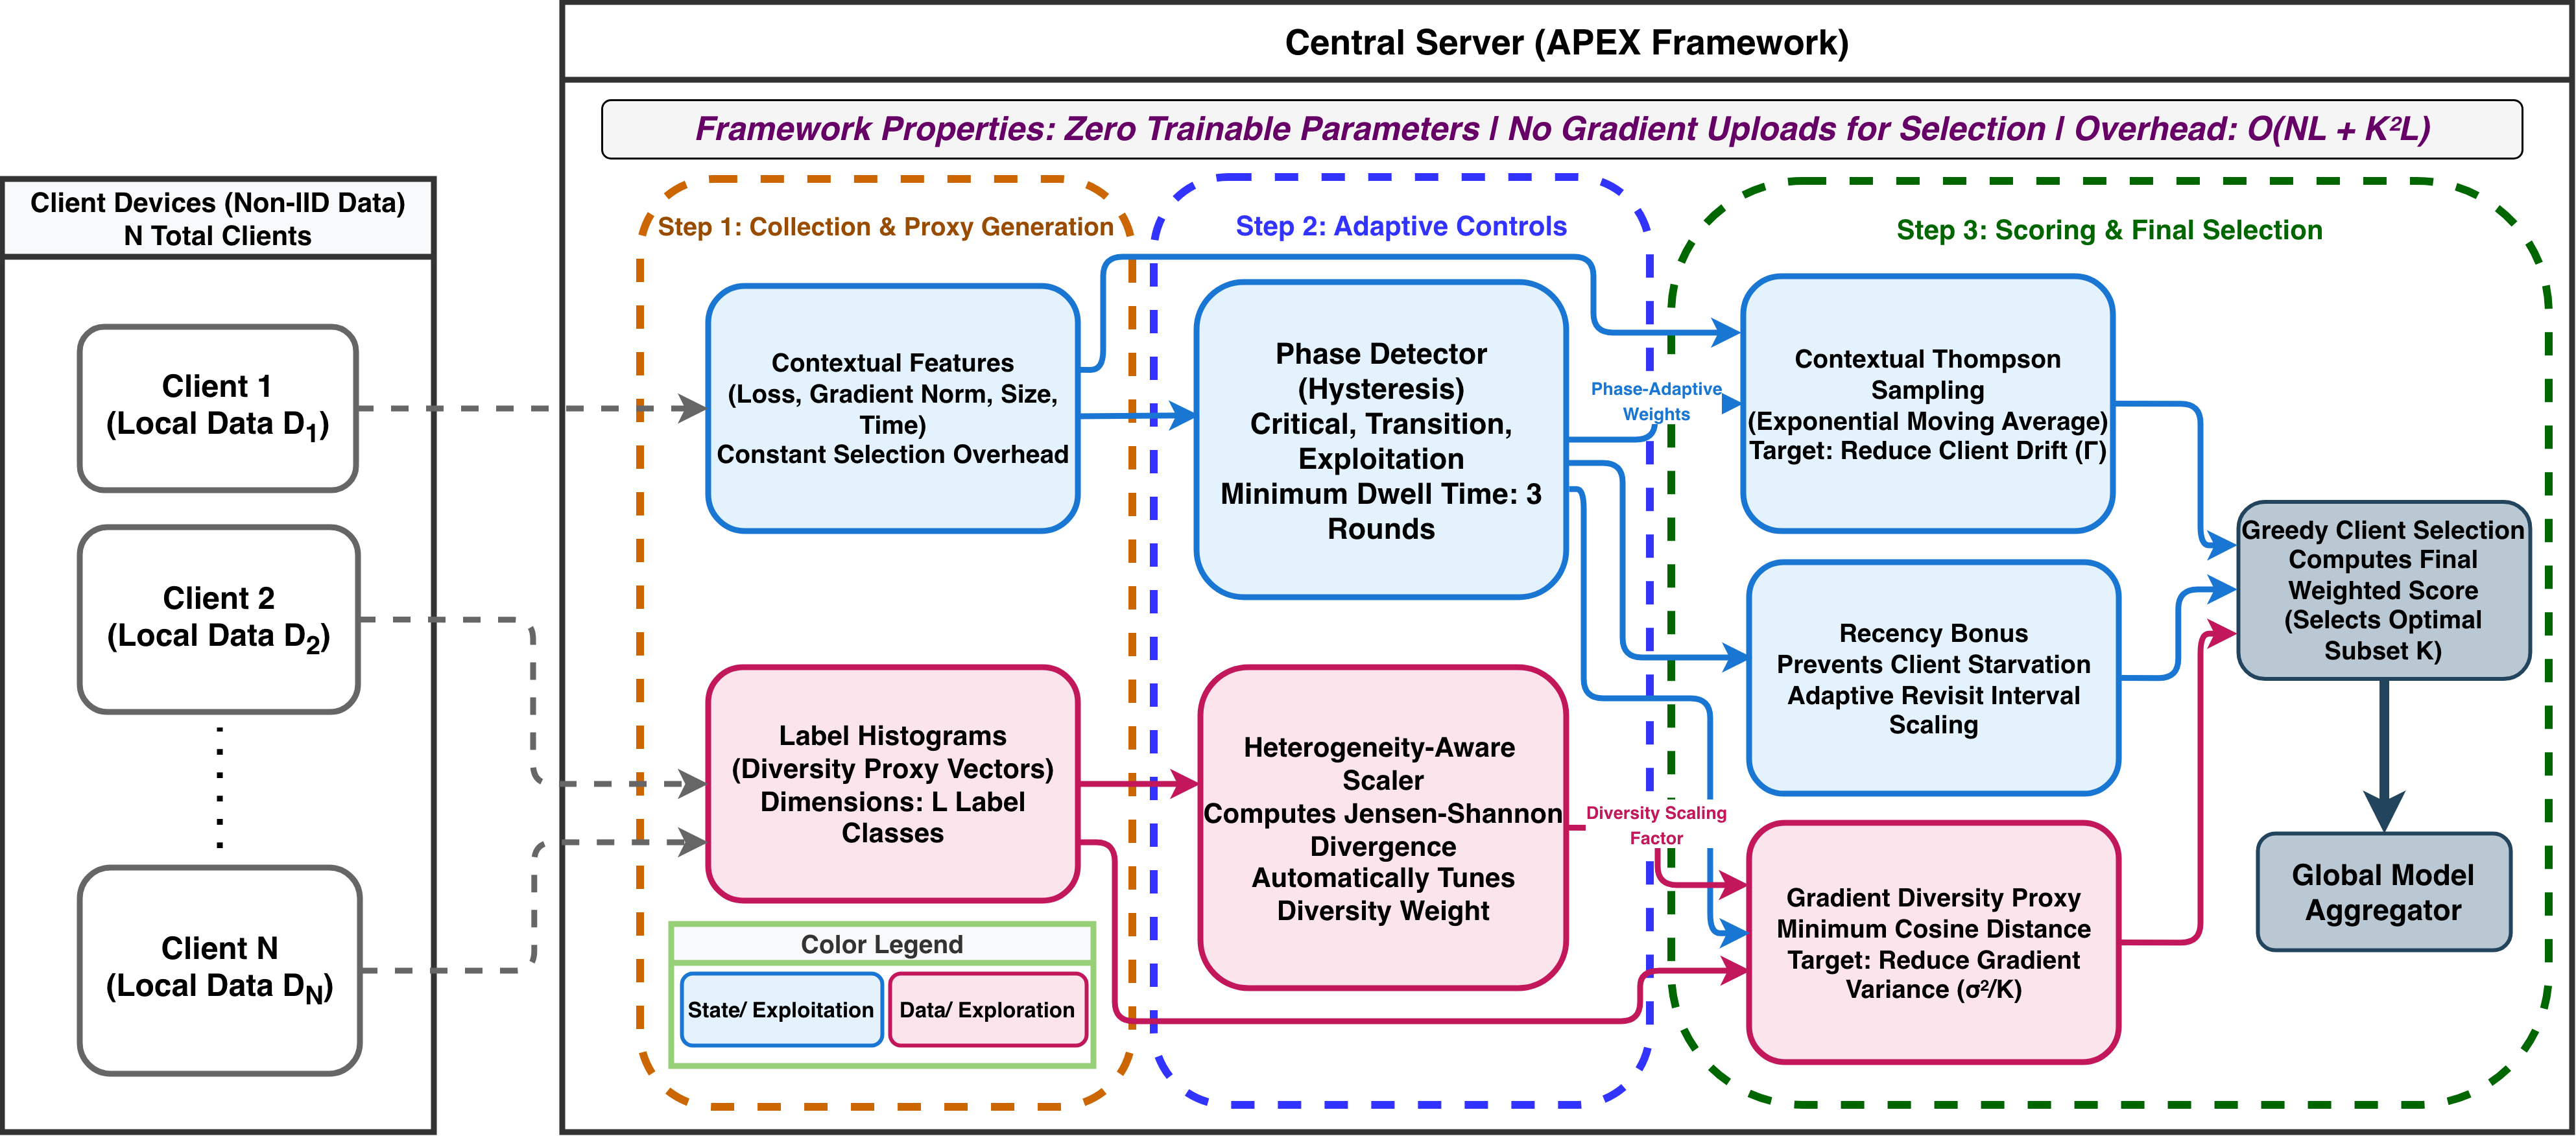
\includegraphics[width=0.95\textwidth]{final_apex_infographic.png}
\caption{System model of the proposed APEX framework. The central server broadcasts the global model $\bm{w}_t$ to $K$ selected clients, which train locally on their non-IID data and upload updated parameters. The APEX selection engine uses the loss history to detect the training phase and combines Thompson sampling, a diversity proxy, and a recency bonus with phase-adaptive weights to select $|\mathcal{S}_t| = K$ clients per round.}
\label{fig:system_model}
\end{figure*}

\subsection{Phase Detection with Hysteresis}

In \cite{yan2023criticalfl}, it has been shown that FL training exhibits critical learning periods where gradient errors cause large and irrecoverable accuracy drops. Based on this, APEX detects the current training phase online using the loss trajectory. The server maintains a sliding window of size $W$ containing the global average loss from recent rounds. Let $\bar{L}_{\text{old}}$ and $\bar{L}_{\text{new}}$ denote the mean loss over the older and newer halves of the window, respectively. Let $\sigma_{\text{rw}}$ denote the standard deviation of the loss values in the recent half. Two statistics are computed from these. The relative improvement rate is given by
\begin{equation}
\rho = \frac{\bar{L}_{\text{old}} - \bar{L}_{\text{new}}}{\bar{L}_{\text{old}} + \epsilon},
\label{eq:rate}
\end{equation}
where $\epsilon$ is a small constant to prevent division by zero. The coefficient of variation over the recent half can be written as
\begin{equation}
\nu = \frac{\sigma_{\text{rw}}}{\bar{L}_{\text{new}} + \epsilon}.
\label{eq:cv}
\end{equation}

The training phase is then classified as follows:
\begin{itemize}
    \item \textit{Critical phase}: $\rho > \tau_c$ and $\nu > \tau_u$. The loss is decreasing rapidly but with high instability. Gradient diversity is needed to prevent irrecoverable drift.
    \item \textit{Transition phase}: $\rho > \tau_e$ but the critical condition is not met. The loss is decreasing steadily. A balanced selection strategy is used.
    \item \textit{Exploitation phase}: $\rho \leq \tau_e$. The loss has reached a plateau. The algorithm relies on calibrated Thompson posteriors to select high-value clients.
\end{itemize}
Here, $\tau_c$, $\tau_u$, and $\tau_e$ are the critical, instability, and exploitation thresholds, respectively. In all experiments, $\tau_c = 0.05$, $\tau_u = 0.10$, $\tau_e = 0.01$, and $W = 5$.

A hysteresis mechanism is used to prevent rapid switching between phases. The phase detector enforces two rules. First, a minimum dwell time of $\delta_{\min} = 3$ rounds is required before any phase transition is allowed. Second, the detector cannot jump directly between the critical and exploitation phases; it must pass through the transition phase. These two rules prevent the destructive oscillation cycle where the phase flips every round due to the feedback between selection strategy and loss trajectory.

\subsection{Contextual Thompson Sampling with Posterior Regularization}

For each client $i$, a four-dimensional feature vector is constructed as
\begin{equation}
\bm{f}_i = \left[\bar{l}_i, \; \bar{g}_i, \; \bar{s}_i, \; \bar{q}_i\right],
\label{eq:features}
\end{equation}
where $\bar{l}_i$, $\bar{g}_i$, $\bar{s}_i$, and $\bar{q}_i$ are the min-max normalized values of the last training loss, gradient norm, inverse training duration, and local data size, respectively. All four features are available at the server without additional communication. The contextual utility for client $i$ can be expressed as
\begin{equation}
u_i^{\text{ctx}} = w_l \bar{l}_i + w_g \bar{g}_i + w_s \bar{s}_i + w_q \bar{q}_i,
\label{eq:ctx_utility}
\end{equation}
where $w_l = 0.4$, $w_g = 0.2$, $w_s = 0.2$, and $w_q = 0.2$ are fixed weights. The Thompson sampling component maintains a posterior distribution for each client. For a client $i$ with $n_i \geq 2$ observations, the Thompson sample is drawn from a normal distribution as
\begin{equation}
\theta_i \sim \mathcal{N}\!\left(\mu_i, \; \frac{\sigma^2_i}{n_i}\right),
\label{eq:ts_sample}
\end{equation}
where $\mu_i$ and $\sigma^2_i$ are the posterior mean and variance. For clients with fewer than two observations, a Beta prior is used instead.

\textit{Posterior regularization.} A variance floor that decays as $\mathcal{O}(1/\sqrt{n})$ is used to prevent the posteriors from collapsing too early. The floor is given by
\begin{equation}
\sigma^2_{\text{floor}} = \frac{c_f}{\sqrt{\max(n_i, 1)}},
\label{eq:var_floor}
\end{equation}
where $c_f = 0.1$. The posterior variance is set to $\sigma^2_i = \max(\hat{\sigma}^2_i, \sigma^2_{\text{floor}})$, where $\hat{\sigma}^2_i$ is the sample variance. At $n_i = 2$, the floor is $0.071$, which maintains substantial exploration. At $n_i = 50$, it drops to $0.014$, allowing exploitation of well-observed clients.

\textit{EMA-smoothed rewards.} The reward signal used for posterior updates is smoothed using an exponential moving average (EMA). The smoothed reward can be written as
\begin{equation}
\tilde{r}_i^{(t)} = \alpha_e \cdot r_i^{(t)} + (1 - \alpha_e) \cdot \tilde{r}_i^{(t-1)},
\label{eq:ema}
\end{equation}
where $\alpha_e = 0.3$ is the EMA coefficient and $r_i^{(t)}$ is the raw reward for client $i$ at round $t$, defined as the per-client share of the accuracy improvement:
\begin{equation}
r_i^{(t)} = \frac{\Delta \text{Acc}^{(t)}}{|\mathcal{S}_t|}, \quad \Delta \text{Acc}^{(t)} = \text{Acc}^{(t)} - \text{Acc}^{(t-1)},
\label{eq:reward}
\end{equation}
where $\text{Acc}^{(t)}$ is the global test accuracy at round $t$. The improvement is divided equally among the $|\mathcal{S}_t|$ selected clients. This filters out single-round noise in the reward signal.

\textit{Confidence-aware blending.} The contextual utility and Thompson sample are blended using a confidence-aware parameter. The blended score for client $i$ can be given as
\begin{equation}
b_i = (1 - \gamma_i^{\text{eff}}) \cdot u_i^{\text{ctx}} + \gamma_i^{\text{eff}} \cdot \theta_i,
\label{eq:blend}
\end{equation}
where the effective blending weight is given by
\begin{equation}
\gamma_i^{\text{eff}} = \gamma \cdot \left(1 - \frac{1}{1 + n_i}\right).
\label{eq:gamma_eff}
\end{equation}
Here, $\gamma = 0.3$ is the base blending weight. For a new client with $n_i = 0$, $\gamma_i^{\text{eff}} = 0$ and the score is determined entirely by the contextual features. For a well-observed client with $n_i = 10$, $\gamma_i^{\text{eff}} \approx 0.91\gamma$, giving the Thompson sample strong influence.

\subsection{Heterogeneity-Aware Gradient Diversity Proxy}

To approximate gradient diversity without requiring gradient communication, a proxy vector is constructed for each client. For client $i$, the proxy vector is given by
\begin{equation}
\bm{z}_i = \left[\bar{l}_i, \; \bar{g}_i, \; \frac{\bm{h}_i}{\|\bm{h}_i\|_2}\right],
\label{eq:proxy}
\end{equation}
where $\bm{h}_i$ is the label histogram of client $i$ and $\|\bm{h}_i\|_2$ is its $L_2$ norm. The first two components capture the training state, while the normalized histogram captures the data distribution. During greedy selection, the diversity bonus for a candidate client $i$ with respect to the already selected set $\mathcal{S}$ can be written as
\begin{equation}
\text{div}(i, \mathcal{S}) = \min_{j \in \mathcal{S}} \left(1 - \frac{\bm{z}_i^\top \bm{z}_j}{\|\bm{z}_i\| \|\bm{z}_j\|}\right).
\label{eq:div_bonus}
\end{equation}
This is the minimum cosine distance between the candidate and all previously selected clients. A high value indicates that the candidate is different from the current selection. When $\mathcal{S} = \emptyset$ (i.e., the first client in the greedy loop), $\text{div}(i, \mathcal{S})$ is undefined and the selection is based on the Thompson and recency components only.

\textit{Heterogeneity-aware scaling.} The diversity weight is scaled by a heterogeneity estimate computed from the client label distributions. The heterogeneity is estimated as the average pairwise Jensen-Shannon divergence \cite{lin1991divergence} across all client label histograms, and is given by
\begin{equation}
\text{het} = \frac{2}{N(N-1)} \sum_{i < j} \text{JSD}(\bm{h}_i \| \bm{h}_j),
\label{eq:het}
\end{equation}
where $\text{JSD}(\cdot)$ denotes the Jensen-Shannon divergence, normalized to $[0, 1]$. This value is computed once in the first round and cached. The raw diversity weight $w_{\text{div}}^{\text{raw}}$ from the phase detector is then scaled as
\begin{equation}
w_{\text{div}} = w_{\text{div}}^{\text{raw}} \cdot \text{het}.
\label{eq:het_scale}
\end{equation}
The removed weight is redistributed to the Thompson component: $w_{\text{ts}} = w_{\text{ts}}^{\text{raw}} + (w_{\text{div}}^{\text{raw}} - w_{\text{div}})$. Under near-IID conditions ($\alpha = 0.6$, $\text{het} \approx 0.3$), the diversity weight drops from $0.60$ to $0.18$ in the critical phase. Under extreme non-IID ($\alpha = 0.1$, $\text{het} \approx 0.9$), it remains at $0.54$. This removes the need for manual tuning across different heterogeneity levels.

\textit{Privacy consideration.} The diversity proxy requires each client to share its label histogram $\bm{h}_i$ with the server. While the histogram does not reveal individual data samples, it does disclose the class distribution of the client's local dataset. Standard mitigations include local differential privacy, where each client adds calibrated noise before uploading, and histogram coarsening into grouped bin counts. The cosine distance used in (\ref{eq:div_bonus}) is robust to moderate perturbations. In this work, label histograms are shared in the clear; integration with differential privacy mechanisms is left for future investigation.

\subsection{Phase-Adaptive Score Combination}

The three components are combined using phase-dependent weights. In the critical phase, the raw weights are $(w_{\text{ts}}^{\text{raw}}, w_{\text{div}}^{\text{raw}}, w_{\text{rec}}^{\text{raw}}) = (0.20, 0.60, 0.20)$, giving the highest weight to diversity to prevent irrecoverable drift. In the transition phase, the weights are $(0.50, 0.30, 0.20)$, providing a balanced setting. In the exploitation phase, the weights are $(0.70, 0.15, 0.15)$, giving the highest weight to Thompson sampling to select clients with high expected contribution based on calibrated posteriors.

The recency bonus for client $i$ encourages the selection of clients that have not been chosen recently, and is given by
\begin{equation}
\text{rec}_i = \frac{\Delta_i}{\Delta_i + C_{\text{rec}}},
\label{eq:recency}
\end{equation}
where $\Delta_i$ is the number of rounds since client $i$ was last selected and $C_{\text{rec}} = \max(N/K, 3.0)$. The constant $C_{\text{rec}}$ scales with the expected revisit interval $N/K$, so that the recency bonus saturates at the same rate regardless of the pool size. The final score for each candidate client $i$ during greedy selection can be expressed as
\begin{equation}
s_i = w_{\text{ts}} \cdot b_i + w_{\text{div}} \cdot \text{div}(i, \mathcal{S}) + w_{\text{rec}} \cdot \text{rec}_i,
\label{eq:final_score}
\end{equation}
where $b_i$ is the blended Thompson-contextual score from (\ref{eq:blend}), $\text{div}(i, \mathcal{S})$ is the diversity bonus from (\ref{eq:div_bonus}), and $\text{rec}_i$ is the recency bonus from (\ref{eq:recency}). The weights $w_{\text{ts}}$, $w_{\text{div}}$, and $w_{\text{rec}}$ are the heterogeneity-scaled values.

The selection proceeds greedily. At each step, the client with the highest score $s_i$ is added to the selected set $\mathcal{S}$, and the diversity bonuses are recomputed for the remaining candidates. This is repeated until $|\mathcal{S}| = K$.

\subsection{Algorithm Summary}

Algorithm~\ref{alg:apex} summarizes the proposed APEX algorithm. In the first round, when no loss information is available, clients are selected by data-size-weighted random sampling (line~3). From round 2 onward, the Thompson posteriors are updated using EMA-smoothed rewards (lines~5--8), the phase is detected with hysteresis (line~9), features are computed (lines~11--12), and clients are scored and selected greedily (lines~13--21). It can be noted that APEX has zero trainable parameters in the sense that no parameters are updated by gradient descent or backpropagation. The algorithm uses a set of manually specified constants (e.g., phase thresholds, contextual weights, EMA coefficient), but these are fixed across all experiments. The auto-scaled parameters ($C_{\text{rec}}$, $\text{het}$, $\gamma_i^{\text{eff}}$) adapt to the problem setting without manual tuning. The per-client state consists of five floats ($\mu_i$, $\sigma^2_i$, $\alpha_i$, $\beta_i$, $\tilde{r}_i$) and one integer ($n_i$). While these constants are fixed across all experiments without per-setting tuning, a formal sensitivity analysis is left for future work.

\begin{algorithm}[t]
\caption{\small APEX: Adaptive Phase-Aware Exploration}
\label{alg:apex}
\begin{algorithmic}[1]
\small
\renewcommand{\algorithmicrequire}{\textbf{Input:}}
\renewcommand{\algorithmicensure}{\textbf{Output:}}
\REQUIRE Round index $t$, clients per round $K$, client set $\mathcal{C}$, history
\ENSURE Selected client set $\mathcal{S}_t$

\IF{$t = 1$ (no loss information available)}
    \RETURN Data-size-weighted random sample of $K$ clients
\ENDIF

\STATE \textit{// Update Thompson posteriors with EMA-smoothed rewards}
\FOR{each client $i$ in previous selection $\mathcal{S}_{t-1}$}
    \STATE $\tilde{r}_i \leftarrow \alpha_e \cdot r_i + (1 - \alpha_e) \cdot \tilde{r}_i^{\text{prev}}$
    \STATE Update posterior $(\mu_i, \sigma^2_i, n_i)$ using $\tilde{r}_i$
    \STATE $\sigma^2_i \leftarrow \max(\sigma^2_i, \; c_f / \sqrt{n_i})$ \hfill $\triangleright$ Variance floor
\ENDFOR

\STATE Detect phase with hysteresis: $\phi \leftarrow \text{DetectPhase}(\text{loss history})$

\STATE \textit{// Compute features and proxy vectors}
\STATE Compute $\bm{f}_i$ for all $i \in \mathcal{C}$ using (\ref{eq:features})
\STATE Compute $\bm{z}_i$ for all $i \in \mathcal{C}$ using (\ref{eq:proxy})

\STATE \textit{// Score all clients}
\STATE Get raw weights $(w_{\text{ts}}^{\text{raw}}, w_{\text{div}}^{\text{raw}}, w_{\text{rec}}^{\text{raw}})$ for phase $\phi$
\STATE Scale weights by heterogeneity using (\ref{eq:het_scale})
\FOR{each client $i \in \mathcal{C}$}
    \STATE Compute $u_i^{\text{ctx}}$ using (\ref{eq:ctx_utility}), sample $\theta_i$ using (\ref{eq:ts_sample})
    \STATE Compute $b_i$ using (\ref{eq:blend}) with $\gamma_i^{\text{eff}}$ from (\ref{eq:gamma_eff})
    \STATE Compute $\text{rec}_i$ using (\ref{eq:recency})
\ENDFOR

\STATE \textit{// Greedy selection with diversity}
\STATE $\mathcal{S}_t \leftarrow \emptyset$
\FOR{$k = 1$ to $K$}
    \STATE $i^* \leftarrow \arg\max_{i \notin \mathcal{S}_t} \; s_i$ \hfill $\triangleright$ Score from (\ref{eq:final_score})
    \STATE $\mathcal{S}_t \leftarrow \mathcal{S}_t \cup \{i^*\}$
\ENDFOR
\RETURN $\mathcal{S}_t$
\end{algorithmic}
\end{algorithm}

% ============================================================================
% SECTION V: THEORETICAL ANALYSIS
% ============================================================================
\section{Theoretical Analysis}

In this section, we present the theoretical analysis for the proposed APEX algorithm. We first show how the proposed algorithm reduces both terms in the convergence bound from (\ref{eq:convergence_bound}). The regret guarantee of the Thompson sampling component is then discussed, followed by the validity of the phase detection mechanism. A complexity analysis is also provided.

\subsection{Convergence Bound Reduction}

The convergence bound in (\ref{eq:convergence_bound}) contains two terms that depend on the client selection policy: the client drift $\Gamma$ and the gradient variance $\sigma^2/K$. The following remark describes how APEX targets both terms simultaneously.

\textit{Remark 1 (Dual Bound Reduction):} Let the assumptions in (\ref{eq:convergence_bound}) hold. The APEX selection policy targets the reduction of both $\Gamma$ and $\sigma^2/K$ through the following mechanisms:

\begin{enumerate}
    \item[(a)] \textit{Client drift mitigation.} The contextual utility $u_i^{\text{ctx}}$ in (\ref{eq:ctx_utility}) assigns weight $w_l = 0.4$ to the training loss. Combined with the Thompson sampling component, this produces a loss-biased selection that prioritizes clients with high training loss, making faster per-round progress despite the client drift $\Gamma$. This is the same mechanism that gives Power-of-Choice its $3\times$ convergence speedup \cite{cho2022towards}.

    \item[(b)] \textit{Gradient variance reduction.} The diversity proxy in (\ref{eq:div_bonus}) selects clients with complementary label distributions. When aggregated, diverse gradients cancel component-wise noise, reducing the effective gradient variance. In \cite{balakrishnan2022diverse}, submodular gradient selection reduces the variance term by $\mathcal{O}(1/K)$. APEX approximates this effect using a lightweight label-histogram-based proxy without gradient communication. This is consistent with the analysis in \cite{zhang2026fednkrf}, where excess risk bounds with minimax optimal rates are derived under data heterogeneity.
\end{enumerate}

The phase-adaptive weights control the relative emphasis: in the critical phase, the diversity component receives higher weight to mitigate the $\sigma^2/K$ term, while in the exploitation phase, the Thompson component receives higher weight to mitigate the $\Gamma$ term.

\subsection{Regret Guarantee}

\textit{Proposition 2 (Bayesian Regret Bound):} The Thompson sampling component in APEX, with posterior updates as in (\ref{eq:ts_sample}) and variance floor as in (\ref{eq:var_floor}), achieves $\mathcal{O}(\sqrt{NT\log T})$ Bayesian regret over $T$ rounds with $N$ clients \cite{agrawal2012analysis}. This follows from the standard regret analysis for Thompson sampling \cite{agrawal2012analysis}, \cite{chapelle2011empirical}. The contextual utility $u_i^{\text{ctx}}$ is deterministic and contributes zero regret. The diversity and recency components are bounded in $[0, 1]$ and act as bounded perturbations. The Thompson posterior concentrates at rate $\mathcal{O}(1/\sqrt{n_i})$, ensuring convergence to the true client utilities. The posterior regularization in (\ref{eq:var_floor}) preserves this concentration rate since the floor itself decays at $\mathcal{O}(1/\sqrt{n})$.

Two caveats apply. First, APEX selects $K$ clients per round, and the stated bound assumes the $K$-arm selection decomposes into $K$ independent pulls, which is a common simplification in combinatorial bandit analyses. Second, the variance floor in (\ref{eq:var_floor}) may increase the constant factor in the regret bound while preserving the asymptotic order.

\subsection{Phase Detection Validity}

The phase detection mechanism is motivated by CriticalFL \cite{yan2023criticalfl}, where gradient errors during critical learning periods cause accuracy drops of $10\times$ to $100\times$ the magnitude observed in non-critical periods. The hysteresis mechanism provides two stability properties. First, the minimum dwell time of $\delta_{\min} = 3$ prevents round-to-round oscillation between phases. Second, the no-skip rule requires transitions to pass through the intermediate phase, preventing abrupt strategy changes from full diversity ($w_{\text{div}}^{\text{raw}} = 0.60$) to full exploitation ($w_{\text{ts}}^{\text{raw}} = 0.70$). Without hysteresis, the oscillation cycle leads to accuracy drops exceeding 10 percentage points per round under extreme non-IID conditions ($\alpha = 0.1$), as observed in our experiments.

\subsection{Complexity Analysis}

The total per-round time complexity of APEX is $\mathcal{O}(NK^2L)$. The greedy diversity selection runs $K$ iterations; at iteration $k$, the diversity bonus is computed for all remaining candidates against $k-1$ selected clients, giving $\sum_{k=1}^{K} N(k-1)L = \mathcal{O}(NK^2L)$. The remaining components are all $\mathcal{O}(N)$ or lower. The space complexity is $\mathcal{O}(NL + T)$. The heterogeneity estimation has $\mathcal{O}(N^2)$ cost but is computed once and cached. For the main setting with $N = 50$, $K = 10$, and $L = 10$, the measured overhead is 3.9~ms per round. Compared to DivFL at $\mathcal{O}(N^2d)$, APEX achieves diversity-aware selection at a fraction of the cost since $L \ll d$.

\begin{figure*}[t]
\centering
\includegraphics[width=0.85\textwidth]{figures/fig_multi_panel_v3.pdf}
\caption{Accuracy, loss, F1 score, and fairness Gini on CIFAR-10 with $\alpha = 0.3$, $N = 50$, $K = 10$ over 200 rounds. Results averaged over three independent seeds; shaded region denotes $\pm 1$ standard deviation for APEX.}
\label{fig:convergence}
\end{figure*}

% ============================================================================
% SECTION VI: SIMULATION RESULTS
% ============================================================================
\section{Experimental Results}
In this section, experimental results on four datasets with different heterogeneity levels and client pool sizes are presented to demonstrate the effectiveness of the proposed APEX algorithm.

\subsection{Experimental Setup}

Four image classification datasets are used: CIFAR-10 \cite{krizhevsky2009learning}, CIFAR-100 \cite{krizhevsky2009learning}, MNIST \cite{lecun1998gradient}, and Fashion-MNIST \cite{xiao2017fashionmnist}. For CIFAR-10 and CIFAR-100, a ResNet18 model \cite{he2016deep} is used. For MNIST and Fashion-MNIST, a CNN-MNIST model is used, consisting of two convolutional layers (10 and 20 filters, $5 \times 5$ kernels) with max-pooling, followed by two fully connected layers (50 and 10 units). Non-IID data partitions are generated using the Dirichlet distribution \cite{hsu2019measuring} with $\alpha \in \{0.1, 0.3, 0.6\}$. The number of clients is set to $N \in \{50, 100, 200\}$, with $K = 10$ clients selected per round ($K = 20$ for $N = 200$). Training runs for $T = 200$ rounds with $E = 1$ local epoch, batch size 32, and learning rate $\eta = 0.01$. The proposed method is compared against FedAvg \cite{mcmahan2017communication}, FedCS \cite{nishio2019client}, FedCor \cite{tang2022fedcor}, TiFL \cite{chai2020tifl}, Oort \cite{lai2021oort}, Power-of-Choice (PoC) \cite{cho2022towards}, and MMR-Diverse \cite{carbonara2024mmr}. All experiments are repeated with three independent seeds (42, 123, 456) and results are reported as mean $\pm$ standard deviation.

\subsection{Main Benchmark: CIFAR-10, $\alpha = 0.3$, $N = 50$}

Table~\ref{tab:main_results} summarizes the main benchmark results on CIFAR-10 with $\alpha = 0.3$, $N = 50$, and $K = 10$ over 200 rounds. APEX achieves 70.67\% $\pm$ 1.17\% test accuracy, which is the highest among all eight methods. MMR-Diverse achieves the second-best accuracy at 70.47\% $\pm$ 0.62\%, while FedAvg achieves 69.52\% $\pm$ 0.65\%. A clear performance gap is observed between the top three methods (APEX, MMR-Diverse, FedAvg) and the system-aware methods (Oort, TiFL, FedCS), which trail by 6--10 percentage points. This result indicates that biased system-aware selection, which repeatedly selects fast clients, actively harms model accuracy under non-IID conditions.

\begin{table}[t]
\centering
\caption{Main benchmark results on CIFAR-10 ($\alpha = 0.3$, $N = 50$, $K = 10$, $T = 200$). Results averaged over 3 seeds. Best in bold.}
\label{tab:main_results}
\footnotesize
\renewcommand{\arraystretch}{1.0}
\setlength{\tabcolsep}{2pt}
\begin{tabular}{lcccc}
\toprule
\textbf{Method} & \textbf{Final Acc.} & \textbf{Peak Acc.} & \textbf{F1} & \textbf{Gini} \\
\midrule
\textbf{APEX} & \textbf{.707$\pm$.012} & \textbf{.727$\pm$.003} & .695$\pm$.022 & .19 \\
MMR-Div. & .705$\pm$.006 & .719$\pm$.008 & \textbf{.701$\pm$.018} & .16 \\
FedAvg & .695$\pm$.007 & .713$\pm$.007 & .687$\pm$.009 & \textbf{.08} \\
PoC & .653$\pm$.031 & .670$\pm$.021 & .653$\pm$.035 & .53 \\
FedCor & .647$\pm$.008 & .649$\pm$.010 & .641$\pm$.005 & .74 \\
Oort & .645$\pm$.010 & .655$\pm$.007 & .641$\pm$.011 & .80 \\
TiFL & .639$\pm$.023 & .644$\pm$.019 & .628$\pm$.038 & .80 \\
FedCS & .610$\pm$.044 & .620$\pm$.035 & .596$\pm$.043 & .80 \\
\bottomrule
\end{tabular}
\end{table}

As depicted in Fig.~\ref{fig:convergence}(a), the accuracy convergence is plotted for all methods over 200 rounds. APEX leads in accuracy from round 100 onward, with the separation becoming more pronounced in the final 50 rounds as the Thompson posteriors become well-calibrated. In Fig.~\ref{fig:convergence}(b), the training loss curves show that APEX and FedAvg achieve the lowest final loss, while system-aware methods stagnate above 1.0. Figure~\ref{fig:convergence}(d) indicates that system-aware methods (Oort, TiFL, FedCS) exhibit Gini coefficients above 0.79 throughout training, whereas APEX maintains a Gini below 0.20. Furthermore, APEX achieves the highest peak accuracy (72.69\% $\pm$ 0.27\%) with the lowest variance across seeds, indicating highly reproducible performance.

\subsection{Fairness Analysis}

In Fig.~\ref{fig:fairness}, the relationship between accuracy and participation fairness is presented. It can be witnessed that APEX uniquely occupies the Pareto frontier, achieving the highest accuracy with a Gini coefficient of 0.19. In contrast, system-aware methods (Oort, TiFL, FedCS) exhibit Gini coefficients of 0.80, indicating that they select the same clients in nearly every round. FedAvg achieves the lowest Gini (0.08) due to uniform random selection, but at the cost of lower accuracy. APEX avoids participation concentration through the recency bonus in (\ref{eq:recency}) and the diversity proxy in (\ref{eq:div_bonus}), achieving $4\times$ better fairness than all system-aware baselines without sacrificing accuracy.

\begin{figure}[t]
\centering
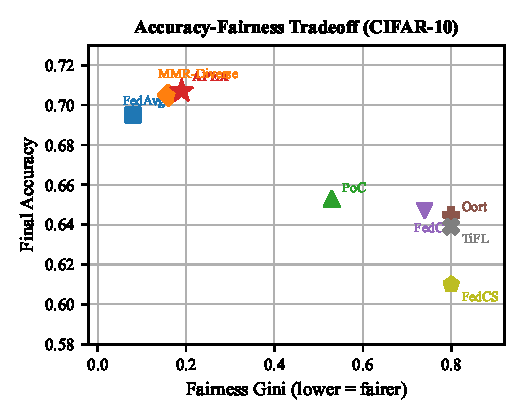
\includegraphics[width=\columnwidth]{figures/apex_analysis/fig06_fairness_accuracy.eps}
\caption{Accuracy versus participation fairness (Gini coefficient, lower is fairer) on CIFAR-10 ($\alpha = 0.3$, $N = 50$). APEX occupies the Pareto frontier, achieving the highest accuracy with near-random fairness.}
\label{fig:fairness}
\end{figure}

\subsection{Heterogeneity Robustness}

In this section, the robustness of APEX across different heterogeneity levels is evaluated. Table~\ref{tab:heterogeneity} presents the results for $\alpha \in \{0.1, 0.3, 0.6\}$ on CIFAR-10.

Table~\ref{tab:heterogeneity} shows that APEX ranks first at all three heterogeneity levels. The advantage of the proposed method is most pronounced under extreme non-IID conditions ($\alpha = 0.1$), where APEX achieves 61.01\% $\pm$ 2.39\%, outperforming FedAvg by 1.88 percentage points and Oort by 14.4 percentage points. It is observed that MMR-Diverse, which achieves the second-best accuracy at $\alpha = 0.3$, degrades to rank four at $\alpha = 0.1$ with a standard deviation of 5.98\%, indicating that pure diversity heuristics become unreliable under extreme label skew. Similarly, Oort drops to 46.60\% at $\alpha = 0.1$ as its loss-based utility becomes unreliable under severe imbalance. These results confirm that the heterogeneity-aware scaling mechanism enables robust performance without manual tuning.

\begin{table}[t]
\centering
\caption{Heterogeneity robustness on CIFAR-10 ($N = 50$, $K = 10$, $T = 200$). Accuracy (mean over 3 seeds) and fairness Gini across three heterogeneity levels.}
\label{tab:heterogeneity}
\footnotesize
\renewcommand{\arraystretch}{1.0}
\setlength{\tabcolsep}{2.5pt}
\begin{tabular}{lcccccc}
\toprule
& \multicolumn{2}{c}{$\alpha = 0.1$} & \multicolumn{2}{c}{$\alpha = 0.3$} & \multicolumn{2}{c}{$\alpha = 0.6$} \\
\cmidrule(lr){2-3} \cmidrule(lr){4-5} \cmidrule(lr){6-7}
\textbf{Method} & \textbf{Acc.} & \textbf{Gini} & \textbf{Acc.} & \textbf{Gini} & \textbf{Acc.} & \textbf{Gini} \\
\midrule
\textbf{APEX} & \textbf{.610} & .19 & \textbf{.707} & .19 & \textbf{.735} & .19 \\
FedAvg & .591 & \textbf{.07} & .695 & \textbf{.08} & .711 & \textbf{.07} \\
PoC & .569 & .53 & .653 & .53 & .679 & .53 \\
MMR-Div. & .541 & .16 & .705 & .16 & .729 & .16 \\
Oort & .466 & .80 & .645 & .80 & .679 & .80 \\
\bottomrule
\end{tabular}
\end{table}

\subsection{Scalability and Cross-Dataset Generalization}

Table~\ref{tab:scale_cross} presents the scalability and cross-dataset generalization results. In the upper panel, APEX ranks first at all three scales. The largest advantage appears at $N = 100$ (+2.45 percentage points over FedAvg), confirming that intelligent selection becomes more critical as the client pool grows faster than the selection budget. In the lower panel, APEX ranks first on CIFAR-10, CIFAR-100, and Fashion-MNIST, and second on MNIST. On MNIST, all methods exceed 97.5\% with a spread of only 0.65 pp, confirming saturation. On CIFAR-100 (100 classes), APEX achieves 33.94\% $\pm$ 0.35\%, outperforming FedAvg by 0.53 pp and Oort by 4.74 pp. The consistent ranking across four datasets validates the generalization of the proposed method.

\begin{table}[t]
\centering
\caption{Scalability across client pool sizes (upper) and cross-dataset generalization (lower) with $\alpha = 0.3$, $K = 10$. Mean accuracy over 3 seeds.}
\label{tab:scale_cross}
\footnotesize
\renewcommand{\arraystretch}{1.0}
\setlength{\tabcolsep}{3pt}
\begin{tabular}{lccccccc}
\toprule
& \multicolumn{3}{c}{\textbf{Scalability}} & \multicolumn{4}{c}{\textbf{Cross-Dataset}} \\
\cmidrule(lr){2-4} \cmidrule(lr){5-8}
\textbf{Method} & $N\!=\!50$ & $N\!=\!100$ & $N\!=\!200$ & C-10 & C-100 & FMNI & MNIS \\
\midrule
\textbf{APEX} & \textbf{.707} & \textbf{.620} & \textbf{.522} & \textbf{.707} & \textbf{.339} & \textbf{.839} & .980 \\
FedAvg & .695 & .595 & .517 & .695 & .334 & .837 & \textbf{.981} \\
Oort & .645 & .516 & .481 & .645 & .292 & .833 & .975 \\
PoC & .653 & .507 & .450 & .653 & .302 & .830 & .978 \\
\bottomrule
\end{tabular}
\end{table}

\subsection{Convergence Speed}

APEX reaches key accuracy thresholds faster than all baselines. On CIFAR-10 ($\alpha = 0.3$), APEX reaches 60\% at round 85 (FedAvg: 92, Oort: 124) and 70\% at round 173 (FedAvg: 189), requiring 8\% fewer rounds to reach 70\%. On CIFAR-100, APEX reaches 30\% eight rounds ahead of FedAvg. Only APEX, MMR-Diverse, and FedAvg surpass 70\% on CIFAR-10 within 200 rounds; all system-aware methods plateau below 65\%.

\subsection{Component Analysis}

To assess the stability contribution of each component, five variants, each removing one component, are evaluated on CIFAR-10 with $\alpha = 0.3$, $N = 50$, and $K = 10$. Table~\ref{tab:ablation} presents the results. Since $\alpha = 0.3$ is the most benign heterogeneity level in the evaluation suite, the analysis emphasizes stability and variance behavior rather than mean accuracy gains.

\begin{table}[t]
\centering
\caption{Ablation study on CIFAR-10 ($\alpha = 0.3$, $N = 50$, $K = 10$, $T = 200$). Mean $\pm$ std over 3 seeds.}
\label{tab:ablation}
\footnotesize
\renewcommand{\arraystretch}{1.0}
\setlength{\tabcolsep}{2.5pt}
\begin{tabular}{lccc}
\toprule
\textbf{Variant} & \textbf{Final Acc.} & \textbf{Peak Acc.} & \textbf{Std} \\
\midrule
w/o Het-Scaling & \textbf{.714$\pm$.015} & .727$\pm$.002 & .015 \\
w/o Post. Reg. & \textbf{.714$\pm$.011} & \textbf{.729$\pm$.003} & .011 \\
w/o Adap. Recency & .712$\pm$.004 & .728$\pm$.007 & \textbf{.004} \\
w/o Adap. Gamma & .704$\pm$.004 & .729$\pm$.002 & \textbf{.004} \\
APEX (Full) & .694$\pm$.015 & .725$\pm$.004 & .015 \\
w/o Hysteresis & .693$\pm$.039 & .726$\pm$.004 & .039 \\
\bottomrule
\end{tabular}
\end{table}

Table~\ref{tab:ablation} shows that removing four of the five components yields higher mean final accuracy than the full algorithm under this benign setting. This is expected: heterogeneity-aware scaling, posterior regularization, adaptive recency, and adaptive gamma target stressors such as extreme label imbalance ($\alpha \leq 0.1$), large client pools ($N \geq 100$), and high inter-seed variance, which $\alpha = 0.3$ does not fully impose. Under benign conditions, the regularization these components introduce slightly constrains the search space without a compensating benefit. Importantly, the peak accuracy across all six variants lies within 72.5--72.9\%, confirming that no component degrades the performance ceiling. Removing phase hysteresis is the only variant that reduces final accuracy ($-0.09$ pp) while tripling the seed standard deviation from 0.015 to 0.039, identifying it as the dominant stability mechanism.

Indirect evidence for the remaining components comes from the harder settings already reported: APEX leads FedAvg by 1.88 pp at $\alpha = 0.1$ (Table~\ref{tab:heterogeneity}), where heterogeneity-aware scaling activates, and by 2.45 pp at $N = 100$ (Table~\ref{tab:scale_cross}), where posterior regularization and adaptive recency become more relevant. A dedicated component analysis at these settings is left for an extended version of this work. The accuracy change from removing each component is depicted in Fig.~\ref{fig:ablation}.

\begin{figure}[t]
\centering
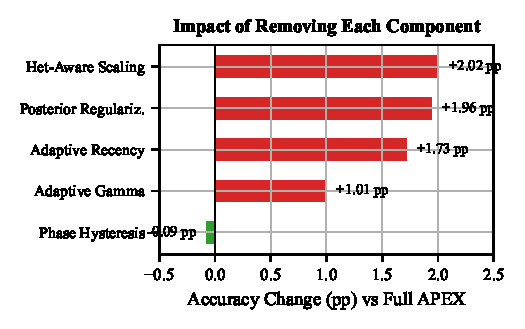
\includegraphics[width=0.92\columnwidth]{figures/apex_analysis/fig10b_ablation_delta.eps}
\caption{Accuracy change from removing each APEX component ($\alpha = 0.3$, $N = 50$, $K = 10$). Positive bars indicate components whose removal slightly improves accuracy under this benign setting; these components are designed to activate under the harder conditions reported in Tables~III and~IV. The negative bar (phase hysteresis) indicates the dominant stability mechanism.}
\label{fig:ablation}
\end{figure}

\subsection{Discussion}

In summary, APEX ranks first in 8 out of 9 experimental settings across four datasets, three heterogeneity levels, and three federation scales; the only exception is MNIST, where the ceiling effect prevents any method from demonstrating a meaningful advantage. The component analysis in Section~VI-G isolates phase hysteresis as the dominant stability mechanism, with the remaining components providing targeted robustness whose effect is masked under benign heterogeneity. The advantage is largest in the most challenging settings: +14.4 pp over Oort at $\alpha = 0.1$ and +2.45 pp over FedAvg at $N = 100$. APEX requires 3.9~ms per round (${\sim}10\times$ less than FedCor). A limitation is elevated seed variance under near-IID conditions, which is expected since the heterogeneity-aware components have no useful signal when data is homogeneous.

% ============================================================================
% SECTION VII: CONCLUSION
% ============================================================================
\section{Conclusion}

In this paper, we have proposed APEX, a lightweight phase-aware client selection algorithm for federated learning under non-IID data heterogeneity. The proposed method combines contextual Thompson sampling with posterior regularization, a label-histogram-based diversity proxy, and a phase detector with hysteresis to target both client drift and gradient variance in the convergence bound. A Jensen-Shannon divergence-based scaling mechanism self-calibrates the diversity weight to the observed heterogeneity level, requiring zero trainable parameters and $\mathcal{O}(NK^2L)$ per-round complexity. Experimental results on four datasets demonstrate that APEX ranks first among eight methods in 8 out of 9 settings, with $4\times$ better participation fairness than system-aware baselines, and the advantage is most pronounced under extreme heterogeneity ($\alpha = 0.1$), where APEX outperforms Oort by 14.4 percentage points.

% ============================================================================
% SECTION VIII: FUTURE WORK
% ============================================================================
\section{Future Work}

Several directions for future work are identified. First, extending the framework to heterogeneous model architectures would allow APEX to operate where client devices differ significantly in computational capability. Second, a formal privacy analysis under local differential privacy for the label histogram proxy is needed, since clients currently share lightweight label distribution summaries with the server. Third, adapting the phase detection mechanism to asynchronous FL settings is a promising direction, as the synchronous round-based design may not scale to environments with highly variable client availability.

% \IEEEtriggeratref{24}
\bibliographystyle{IEEEtran}
\bibliography{references}

\end{document}
